% ===================================================================
% SKILL: TIKZ GRAFİK VE GÖRSELLEŞTİRME PRENSİPLERİ
% ===================================================================
% TANIM:
% Bu dosya, LaTeX/Beamer'da TikZ kullanarak grafik çizerken uyulması
% gereken "Altın Kuralları" ve "Güvenli Şablonları" içerir.
% 
% TEMEL İLKELER (LLM İÇİN YÖNERGE):
% 1. ASLA 3D ÇİZME: TikZ 3D çizimlerde (özellikle perspektif ve gölge)
%    yetersizdir ve görsel kaos yaratır. Her zaman "2D ama 3D gibi
%    anlaşılan" (pseudo-3D) veya düz 2D çizimler tercih edilmelidir.
% 2. METİN ÇAKIŞMASINI ÖNLE: Etiketleri (node) yerleştirirken manuel
%    koordinat yerine "relative positioning" (sağında, üstünde vb.)
%    kullanılmalıdır. 
% 3. BASİTLİK: Gölgelendirme, gradient ve karmaşık efektlerden kaçın.
% ===================================================================

\begin{frame}{TikZ Grafik Örnekleri}
    \begin{columns}[T]
        
        % ÖRNEK 1: BASİT 2D SÜTUN GRAFİĞİ (BAR CHART)
        % Grid, Eksenler ve Çubukların net ayrımı
        \column{0.48\textwidth}
        \centering
        \textbf{Doğru: Temiz 2D Bar Chart}
        \vspace{0.5em}
        
        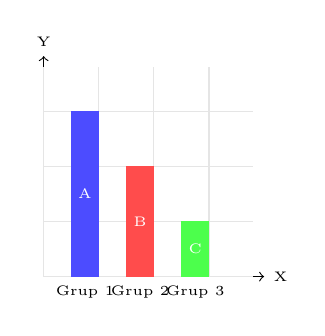
\begin{tikzpicture}[scale=0.7]
            % Eksenler
            \draw[->] (0,0) -- (0,4) node[above] {\tiny Y};
            \draw[->] (0,0) -- (4,0) node[right] {\tiny X};
            
            % Grid (Yardımcı Çizgiler) - Okunabilirliği artırır
            \draw[gray!20, step=1] (0,0) grid (3.8, 3.8);
            
            % Çubuklar (Koordinat hesabı basittir)
            \fill[blue!70] (0.5,0) rectangle (1.0, 3.0) node[midway, white] {\tiny A};
            \fill[red!70]  (1.5,0) rectangle (2.0, 2.0) node[midway, white] {\tiny B};
            \fill[green!70](2.5,0) rectangle (3.0, 1.0) node[midway, white] {\tiny C};
            
            % Etiketlerin çakışmaması için "node[below]" kullanımı
            \node[below] at (0.75, 0) {\tiny Grup 1};
            \node[below] at (1.75, 0) {\tiny Grup 2};
            \node[below] at (2.75, 0) {\tiny Grup 3};
        \end{tikzpicture}

        % ÖRNEK 2: DAĞILIM GRAFİĞİ (SCATTER PLOT)
        % Noktalar ve Trend Çizgisi
        \column{0.48\textwidth}
        \centering
        \textbf{Doğru: Temiz Scatter Plot}
        \vspace{0.5em}
        
        \begin{tikzpicture}[scale=0.7]
            \draw[<->] (0,4) node[left] {\tiny Y} -- (0,0) -- (4,0) node[below] {\tiny X};
            
            % Veri Noktaları (Loop ile temiz kod)
            \foreach \x/\y in {0.5/1, 1.2/1.5, 2.0/2.8, 3.5/3.5} {
                \fill[purple] (\x,\y) circle (2.5pt);
            }
            
            % Etiket Çakışmasını Önleme:
            % Yazıyı noktanın "üstüne" veya "sağına" (anchor) sabitliyoruz.
            \node[right, font=\tiny] at (3.5, 3.5) {Zirve};
            
            % Trend Çizgisi
            \draw[dashed, thick, orange] (0,0.5) -- (4,4);
        \end{tikzpicture}
        
    \end{columns}
\end{frame}

% ÖRNEK 3: AKIŞ ŞEMASI (NODES & ARROWS)
% Metinlerin kutu dışına taşmaması için "text width" kullanımı kritiktir.
\begin{frame}{Akış Şeması (Flowchart)}
    \centering
    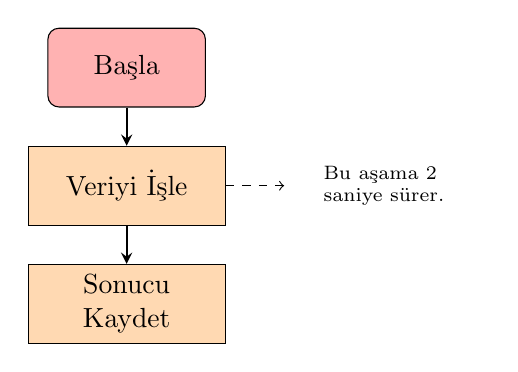
\begin{tikzpicture}[
        node distance=1.5cm,
        % Kutu Stilleri
        startstop/.style={rectangle, rounded corners, minimum width=2cm, minimum height=1cm, text centered, draw=black, fill=red!30},
        process/.style={rectangle, minimum width=2.5cm, minimum height=1cm, text centered, text width=2cm, draw=black, fill=orange!30}, % text width -> Satır atlatır
        arrow/.style={thick,->,>=stealth}
    ]
        % Node Yerleşimi (Relative Positioning)
        \node (start) [startstop] {Başla};
        \node (pro1) [process, below of=start] {Veriyi İşle};
        \node (pro2) [process, below of=pro1] {Sonucu Kaydet};
        
        % Bağlantılar
        \draw[arrow] (start) -- (pro1);
        \draw[arrow] (pro1) -- (pro2);
        
        % Yan Açıklama (Çakışmayı önlemek için xshift)
        \node[right of=pro1, xshift=2cm, font=\scriptsize, text width=2cm] {Bu aşama 2 saniye sürer.};
        \draw[dashed, ->] (pro1) -- +(2,0);
        
    \end{tikzpicture}
\end{frame}
